\subsection{Động lượng}
\begin{frame}
\frametitle{Sự thay đổi chuyển động}
\begin{figure}
    \centering
    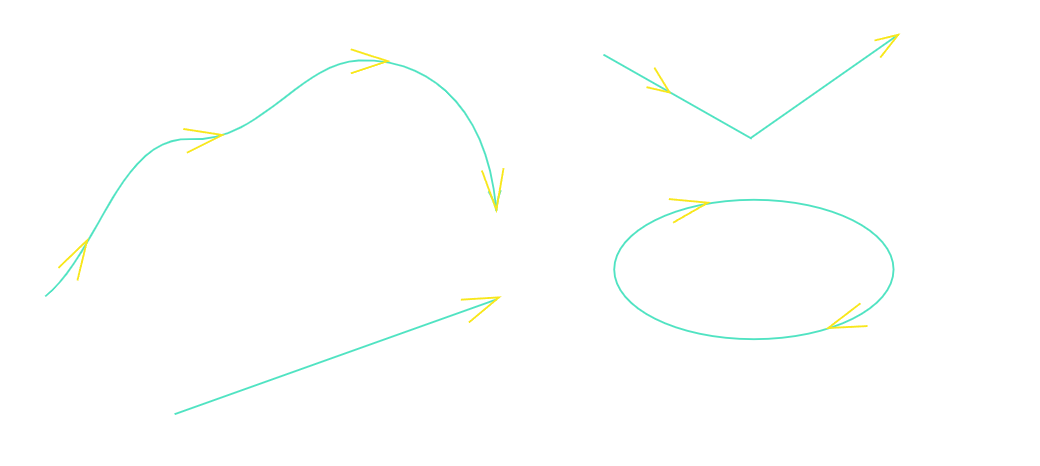
\includegraphics[width=10cm, height =6cm]{Slides/Figure/motionchange.png}
\end{figure}
\end{frame}
\begin{frame}
\frametitle{Tương tác gần và xa (góc nhìn cổ điển)}
\begin{columns}
    \begin{column}{0.5\textwidth}
        \begin{figure}[H]
            \centering
            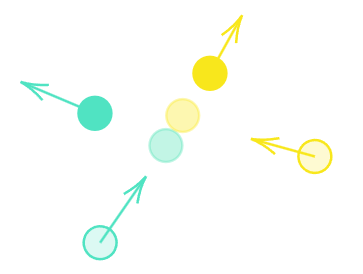
\includegraphics[width=3cm, height=2.5cm]{Slides/Figure/colision1.png}
        \end{figure}
        \begin{figure}[H]
            \centering
            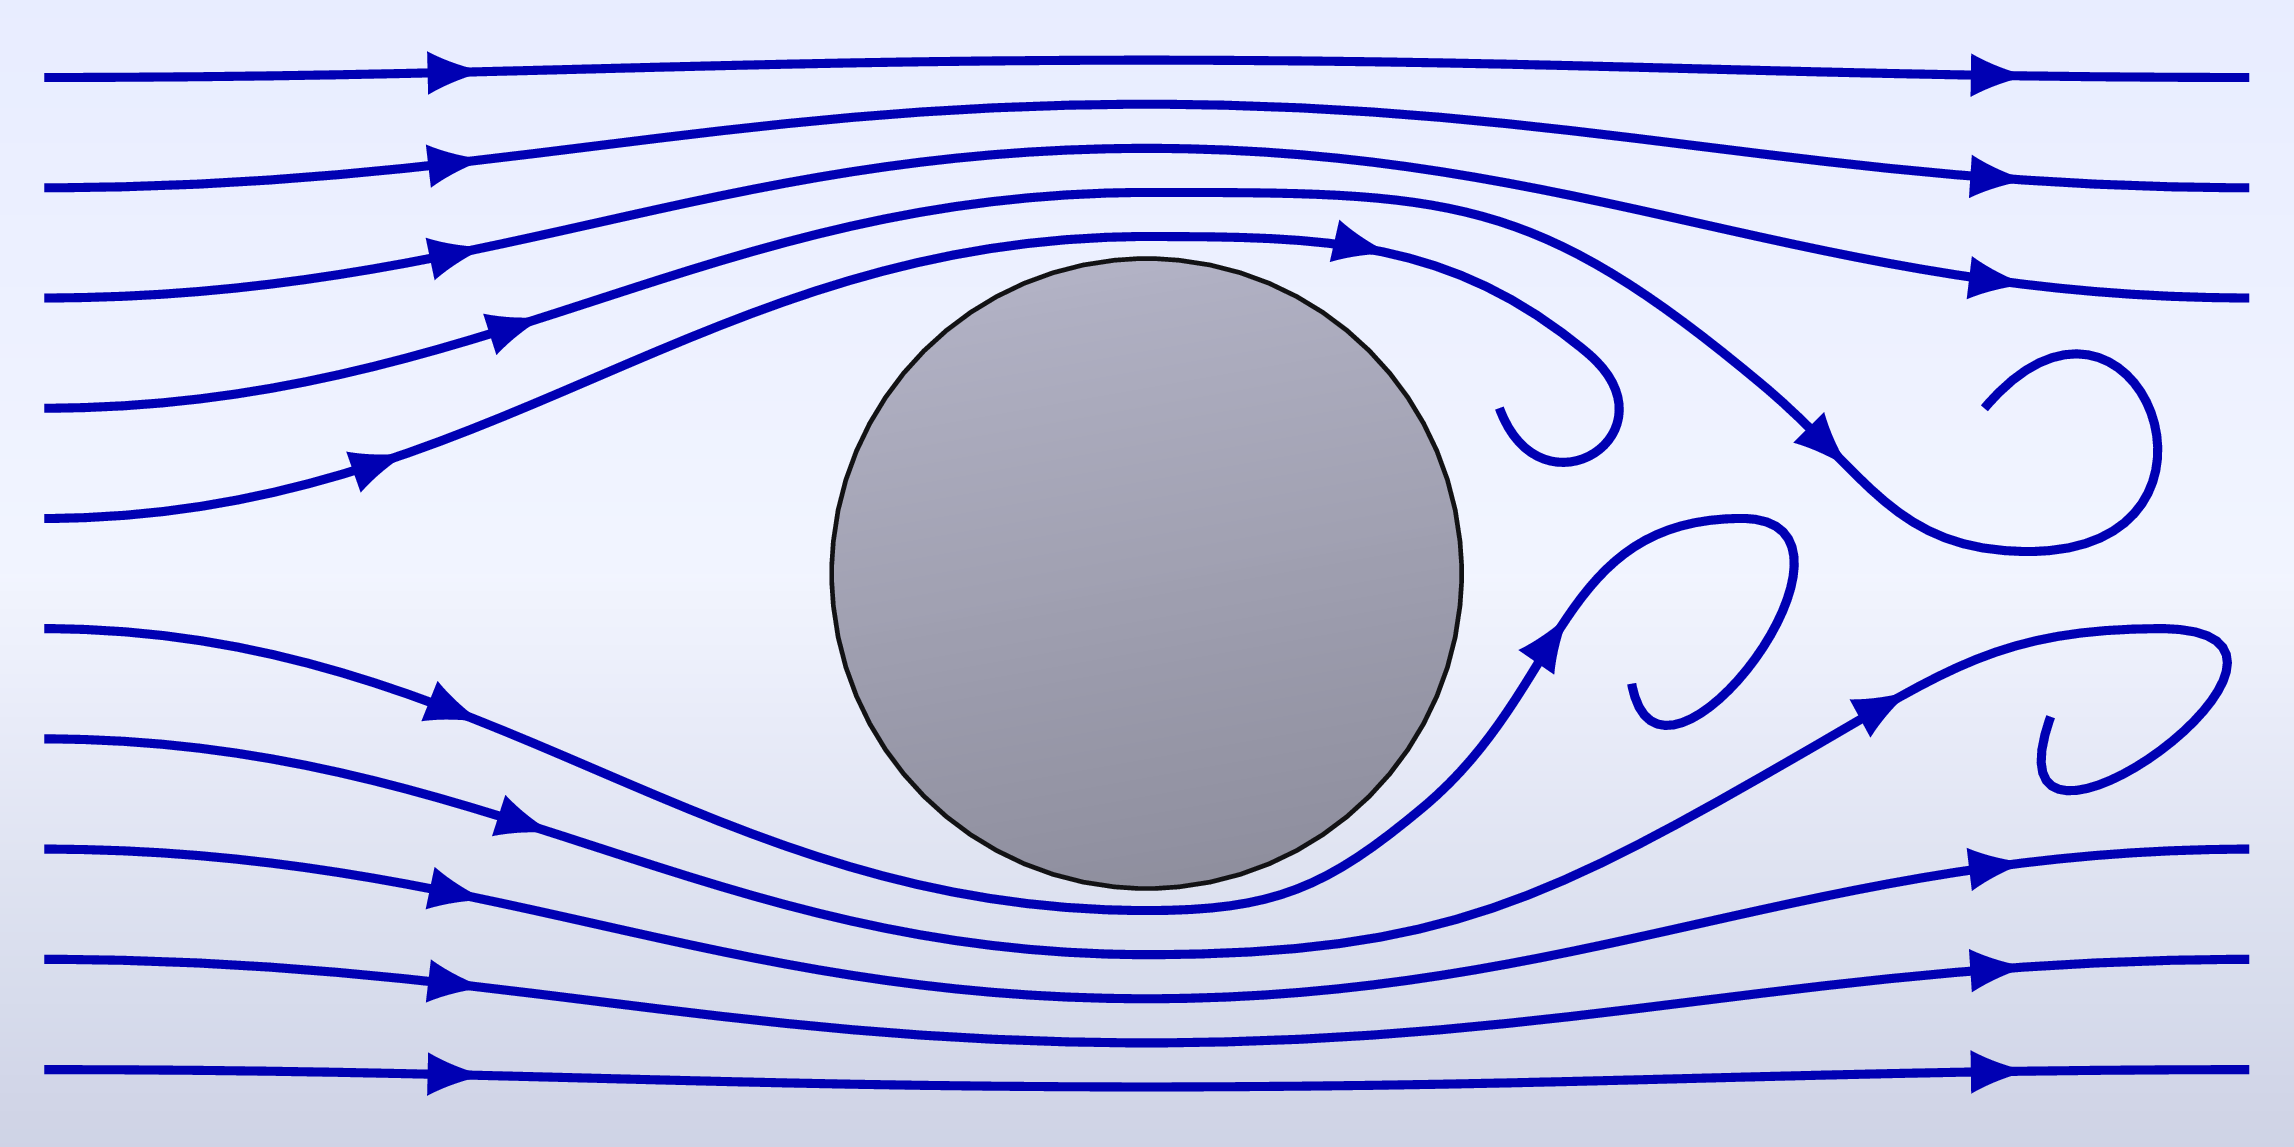
\includegraphics[width=4cm, height=2cm]{Slides/Figure/fluid_dynamics.png}
        \end{figure}
    \end{column}
    \begin{column}{0.5\textwidth}
        \begin{figure}
            \centering
            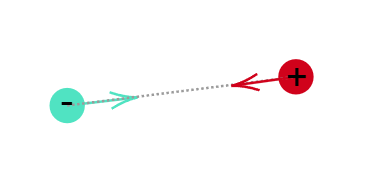
\includegraphics[width=4cm, height=2cm]{Slides/Figure/atraction.png}
        \end{figure}
        \begin{figure}
            \centering
            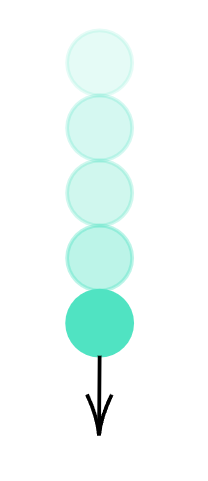
\includegraphics[width=1.5cm, height=3cm]{Slides/Figure/free fall.png}
        \end{figure}
    \end{column}
\end{columns}
\end{frame}
\begin{frame}
    \frametitle{Khối lượng, Động lượng}
    \begin{figure}
        \centering
        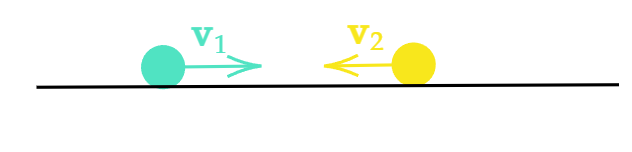
\includegraphics[width=9cm, height=2cm]{Slides/Figure/colision2.png}
    \end{figure}
    \begin{columns}
        \begin{column}{0.3\textwidth}
           Định lượng tính chất của quán tính: \emph{khối lượng}.\newline

            Bảo toàn khối lượng:\[m_1 +m_2 =const.\]
        \end{column}
        \begin{column}{0.3\textwidth}
            Thực nghiệm chứng tỏ \[\frac{\lvert \Delta \mathbf{v}_1 \rvert}{\lvert\Delta\mathbf{v}_2\rvert}=\frac{m_2}{m_1}.\]
            Dạng vector: \[m_1\Delta\mathbf{v}_1 =-m_2\Delta\mathbf{v}_2.\]
        \end{column}
        \begin{column}{0.3\textwidth}
            Động lượng: \[\mathbf{p}=m\mathbf{v}.\]
            Bảo toàn động lượng:
            \[\Delta(\mathbf{p}_1+\mathbf{p}_2)=\mathbf{0}.\]
        \end{column}
    \end{columns}
\end{frame}
\subsection{Nguyên lý tương đối}
\begin{frame}
    \frametitle{Nguyên lý tương đối Galilei}
    \begin{tcolorbox}[colback=blue!10, colframe=blue!50!black]
        Mọi hiện tượng cơ học trong những hệ quy chiếu quán tính khác nhau đều xảy ra một cách giống nhau.
    \end{tcolorbox}
    Hay,
     \begin{tcolorbox}[colback=blue!10, colframe=blue!50!black]
        Mọi hiện tượng cơ học đều xảy ra giống nhau trong những hệ quy chiếu mà trong đó gia tốc của một vật là như nhau.
    \end{tcolorbox}
    \emph{Hệ quy chiếu chuyển động thẳng đều trong một hệ quy chiếu quán tính là một hệ quy chiếu quán tính.}
\end{frame}
\begin{frame}
    \frametitle{Ví dụ: các thí nghiệm trên một đoàn tàu}
    \begin{columns}
        \begin{column}{0.5\textwidth}
            Vận tốc \(v=0, a=0m/s^2\):
            \begin{itemize}
                \item \(\frac{\lvert \Delta \mathbf{v}_1 \rvert}{\lvert\Delta\mathbf{v}_2\rvert}=\frac{m_2}{m_1}\).
                \item Quả táo rơi thẳng đứng với thời gian \(\tau\).
            \end{itemize}
            Vận tốc \(v=100m/s , a=0m/s^2\):
            \begin{itemize}
                \item \(\frac{\lvert \Delta \mathbf{v}_1 \rvert}{\lvert\Delta\mathbf{v}_2\rvert}=\frac{m_2}{m_1}\).
                \item Quả táo rơi thẳng đứng với thời gian \(\tau\).
            \end{itemize}
        \end{column}
          \begin{column}{0.5\textwidth}
            Gia tốc \(a=2m/s^2\):
            \begin{itemize}
                \item \(\frac{\lvert \Delta \mathbf{v}_1 \rvert}{\lvert\Delta\mathbf{v}_2\rvert}\neq\frac{m_2}{m_1}\).
                \item Quả táo rơi chéo với thời gian \(\tau\).
            \end{itemize}
            Vậy, gia tốc với tương tác vật lý có liên hệ gì?
        \end{column}
    \end{columns}
\end{frame}